%-------------------------------------------------
%	Version: 0.0
%	fecha de entrega
%
%-------------------------------------------------

\documentclass[11pt]{report}

%packages
\usepackage{graphicx}
\usepackage{subcaption}

\usepackage[utf8]{inputenc}
\usepackage[spanish, es-nodecimaldot]{babel}
\usepackage{setspace}
\usepackage{ragged2e}

\usepackage{amsmath}
\usepackage{amsthm}
\usepackage{amssymb}
\usepackage{mathtools}
\usepackage{siunitx}
\usepackage[thinc]{esdiff} %derivadas faciles
\usepackage{physics} %algunos simbolos de derivadas

%path donde se encuentran las imagenes
\graphicspath{ {./figuras/} }

%---------------------------------------------------------------
%ABREVIACIONES DE COMANDOS

\theoremstyle{plain}
\newtheorem{thm}{Teorema}[chapter] % reset theorem numbering for each chapter

\theoremstyle{definition}
\newtheorem{defn}[thm]{Definición} % definition numbers are dependent on theorem numbers
\newtheorem{exmp}[thm]{Ejemplo} % same for example numbers

\newcommand{\chaptercontent}{
\section{Basics}
\begin{defn}Here is a new definition.\end{defn}
\begin{thm}Here is a new theorem.\end{thm}
\begin{thm}Here is a new theorem.\end{thm}
\begin{exmp}Here is a good example.\end{exmp}
\subsection{Some tips}
\begin{defn}Here is a new definition.\end{defn}
\section{Advanced stuff}
\begin{defn}Here is a new definition.\end{defn}
\subsection{Warnings}
\begin{defn}Here is a new definition.\end{defn}
}

\usepackage{biblatex}
%\addbibresource{Tarea1.bib}

\begin{document}

\begin{titlepage}
\title{Titulo_del_trabajo}

%-------------------------------------------------
%PORTADA
%-------------------------------------------------

	\centering
	{\scshape\LARGE Universidad Autónoma de Yucatán  \\ Facultad de ingeniería\par}
	\vspace{1cm}
	{\scshape\Large Fenómenos de transporte\par}
	\vspace{1.5cm}
	{\huge\bfseries Apuntes de clase\par}
	\vspace{0.7cm}
	{\begin{figure}[!h]
	\centering
    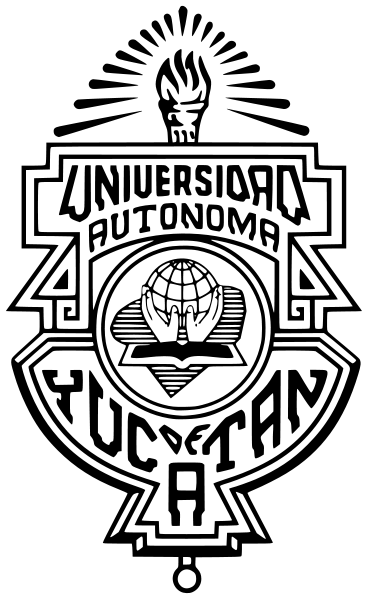
\includegraphics[scale=0.3]{UADY.png}
	\end{figure}}
	\vspace{0.7cm}
	{\Large\itshape Erick Al. Casanova Cortés\par}
	{\Large\itshape Matricula: \par}
	\vfill
	{\scshape\Large Docente\par
	Nombre del docente\par}
	\vfill
	{\Large{\bfseries Fecha de modificacion: \today} }

	\vfill
	
\end{titlepage}

%-------------------------------------------------
%Inicio del documento
%-------------------------------------------------

\tableofcontents

%-------------------------------------------------
%Introducción y conceptos básicos
%-------------------------------------------------
\chapter{Introducción y conceptos básicos}

%---> Formativa <-----
\section{Formativa}
Exámenes (3) 35 \% \\
ADAS (11) 25 \% \\
Proyecto (4) 40 \% \\

\section{Fechas importantes}

Primer parcial 19 abril (conducción) \\
Segundo parcial 3 junio (convección) \\ 
Tercer parcial 1 julio \\

\section{ADAs}
Constan de la resolución de problemas similares a lo que vienen en el examen:\\

\textbf{Características}\\
Carátula escrita en procesador de texto.\\
Resolución de problemas a mano en hojas blancas.\\
Tarea en formato PDF, escaneada con muy buena calidad.\\
Se solicitan y entregan por medio de la plataforma TEAMS.\\
Nombre del archivo ADA\#\_FdT\_CasanovaCortésErickAlejando\\


\section{Proyectos}

\textbf{Primer proyecto}\\
Uso del software Wolfram para determinar el transporte de energía por conducción a nano-escala en ferrofluidos\footnote{Suspensión coloidal estable de nanopartículas de magnetita}.\\


\textbf{Segundo proyecto}\\
Transferencia de calor en estado estacionario en aljibes diatermicos, usando el fusion 360, dibujo de modelos en 3D y simulaciones térmicas.\\


\textbf{Tercer proyecto}\\
Diseño de una madre.\\


\textbf{Cuarto proyecto}\\
Otra shingadera.\\


%-------------------------------------------------
%Conducción de calor
%-------------------------------------------------
\chapter{Conducción de calor}
\section{Introducción a la conducción del calor}
\section{Conducción de calor en es estado estacionario}
\section{Conducción de calor en régimen transitorio}


%-------------------------------------------------
%Convección de calor
%-------------------------------------------------
\chapter{Convección de calor}
\section{Fundamentos de la convección}
\section{Convección externa forzada}
\section{Conveccón interna forzada}
\section{Ebullición y condensación}


%-------------------------------------------------
%Radiación de calor
%-------------------------------------------------
\chapter{Radiación de calor}
\section{Fundamentos de la radiación}
\section{Transferencia de calor por radiación}


%-------------------------------------------------
%Transferencia de masa
%-------------------------------------------------
\chapter{Transferencia de masa}
\section{Introducción}
\section{Difusión de masa}
\section{Convección de masa}
\section{Transferencia simultanea de calor y masa}


%-------------------------------------------------
%Final del documento
%-------------------------------------------------

\end{document}
